\documentclass{beamer}
\usepackage{sansmathaccent}
\pdfmapfile{+sansmathaccent.map}
\usepackage{comment}
\usepackage{physics}
\usetheme{Madrid}

\usepackage[utf8]{inputenc}
\usepackage{graphicx}

\title[Rutherford Scattering]{Rutherford Scattering Detection through Gold Foil}
\author{Henry Shackleton}

\begin{document}

\titlepage

\section{Introduction and Theory}

\begin{frame}
  \frametitle{Plum Pudding and Rutherford Models Predict Different Scattering Behavior}
  \begin{columns}
    \begin{column}{0.5\textwidth}
      \begin{center}
      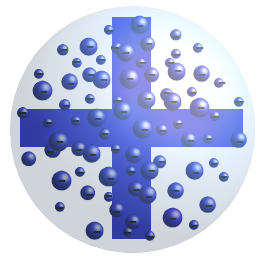
\includegraphics[width=0.5\textwidth]{plum}
      \\
      \textbf{Plum Pudding Model}
      \begin{itemize}
        \pause
        \item Small electrons in a "soup" of positive charge
          \pause
        \item Produces small-angle scattering that dies off exponentially
          \pause
      \end{itemize}
    \end{center}
    \end{column}
    \begin{column}{0.5\textwidth}
      \begin{center}
      \item
        \vspace{-20pt}
      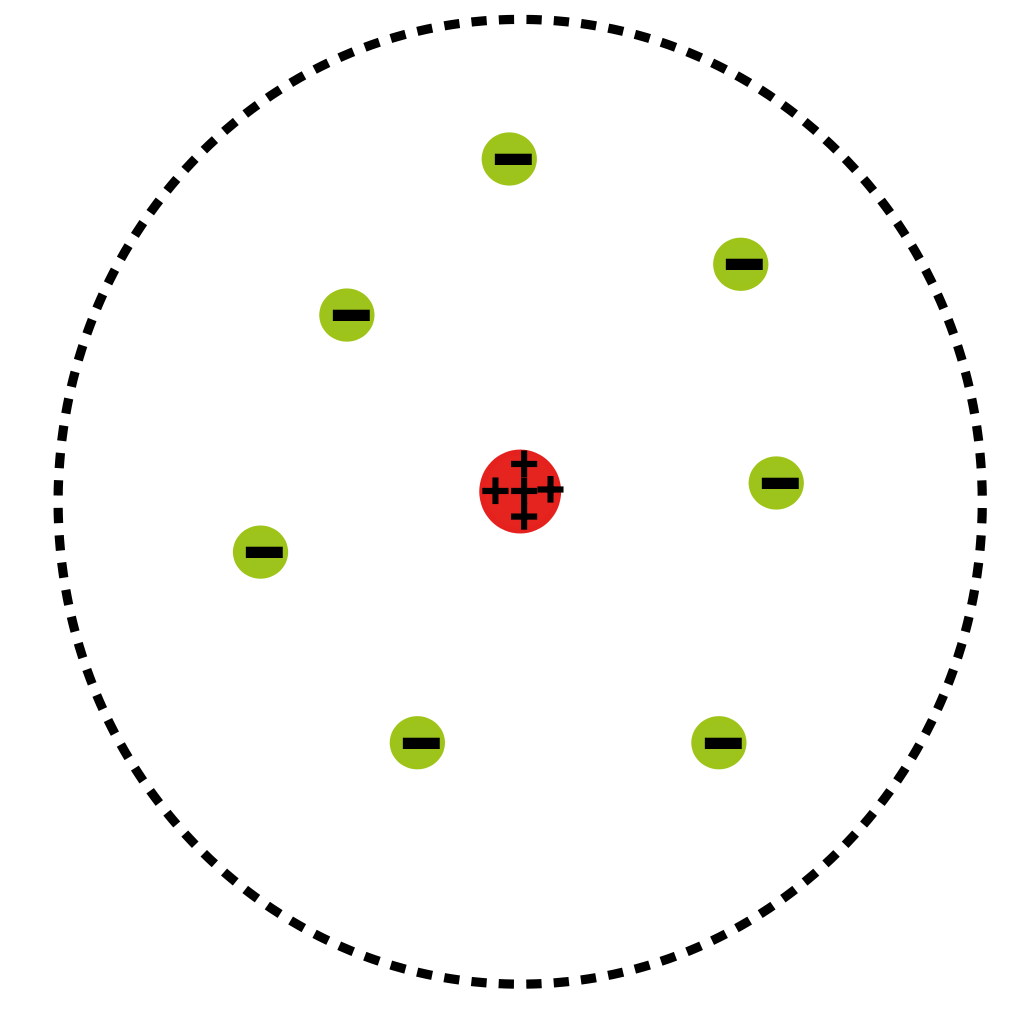
\includegraphics[width=0.44\textwidth]{rutherford.png}
      \\
      \textbf{Rutherford Model}
      \begin{itemize}
        \pause
      \item Electrons surround a concentrated positive charge
        \pause
      \item Allows for large scattering angles
    \end{itemize}
  \end{center}
  \end{column}
\end{columns}
\end{frame}


\begin{frame}
  \frametitle{Rutherford Scattering Derives from Coulumb Interactions}
  \begin{equation*}
    \dv{\sigma}{\Omega} = \left( \frac{Z Z' e^2}{4E}\right)^2 \frac{1}{\sin^4 (\theta/2)}
  \end{equation*}

  \begin{itemize}
    \item Differential cross section describes probability of scattering at angle $\theta$.
    \item Translation to observable trends requires consideration of flux, area density, etc., but does not affect $\theta$-dependence.
    \item Equation only describes \textit{single} scattering events.
  \end{itemize}
\end{frame}

\begin{frame}
  \frametitle{Apparatus allows for scattering detection at various angles}
  \begin{center}
  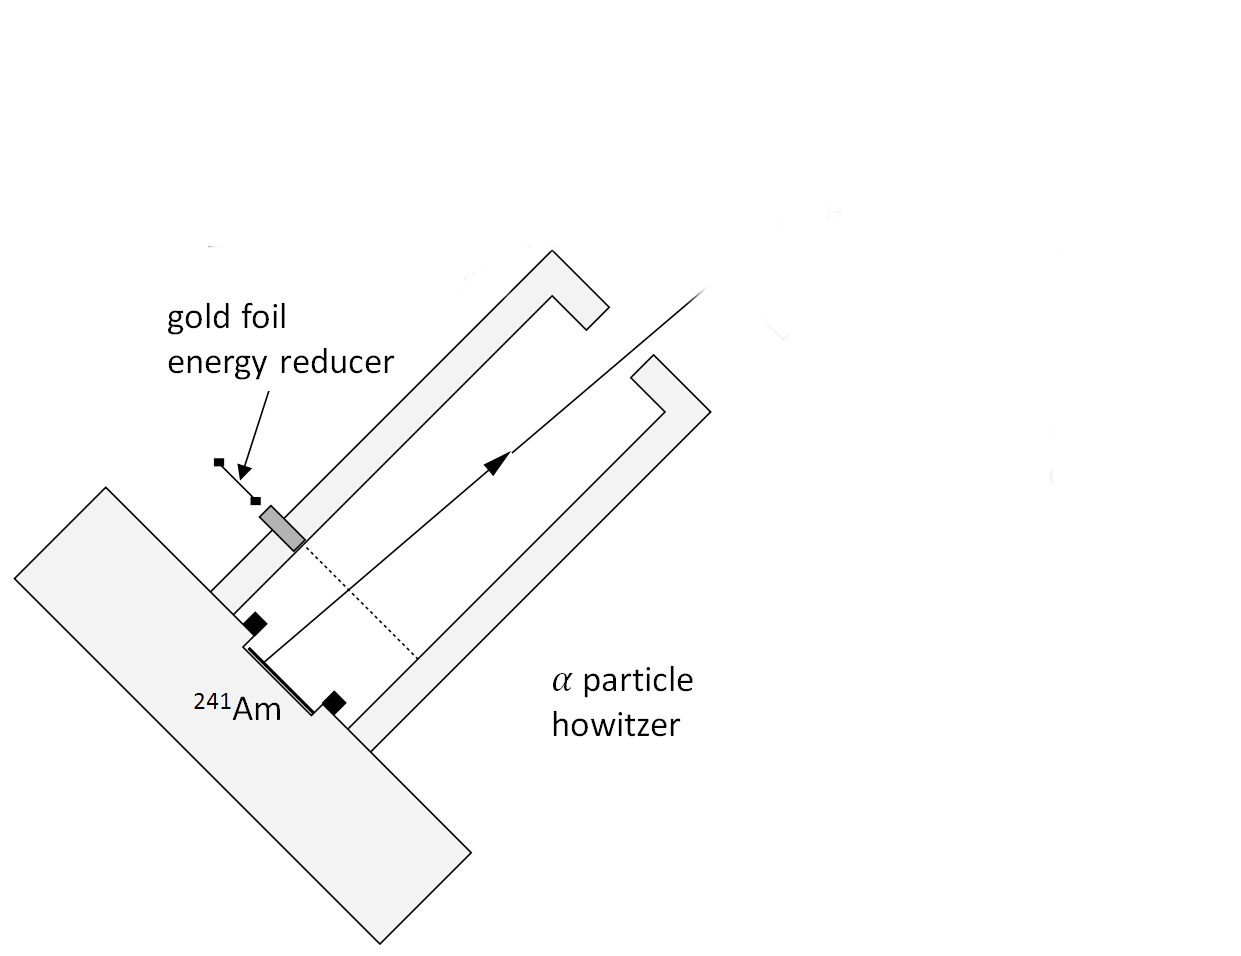
\includegraphics[width=0.8\textwidth]{apparatus-phi-detect-gold}
\end{center}
\end{frame}

\begin{frame}
  \frametitle{Apparatus allows for scattering detection at various angles}
  \begin{center}
  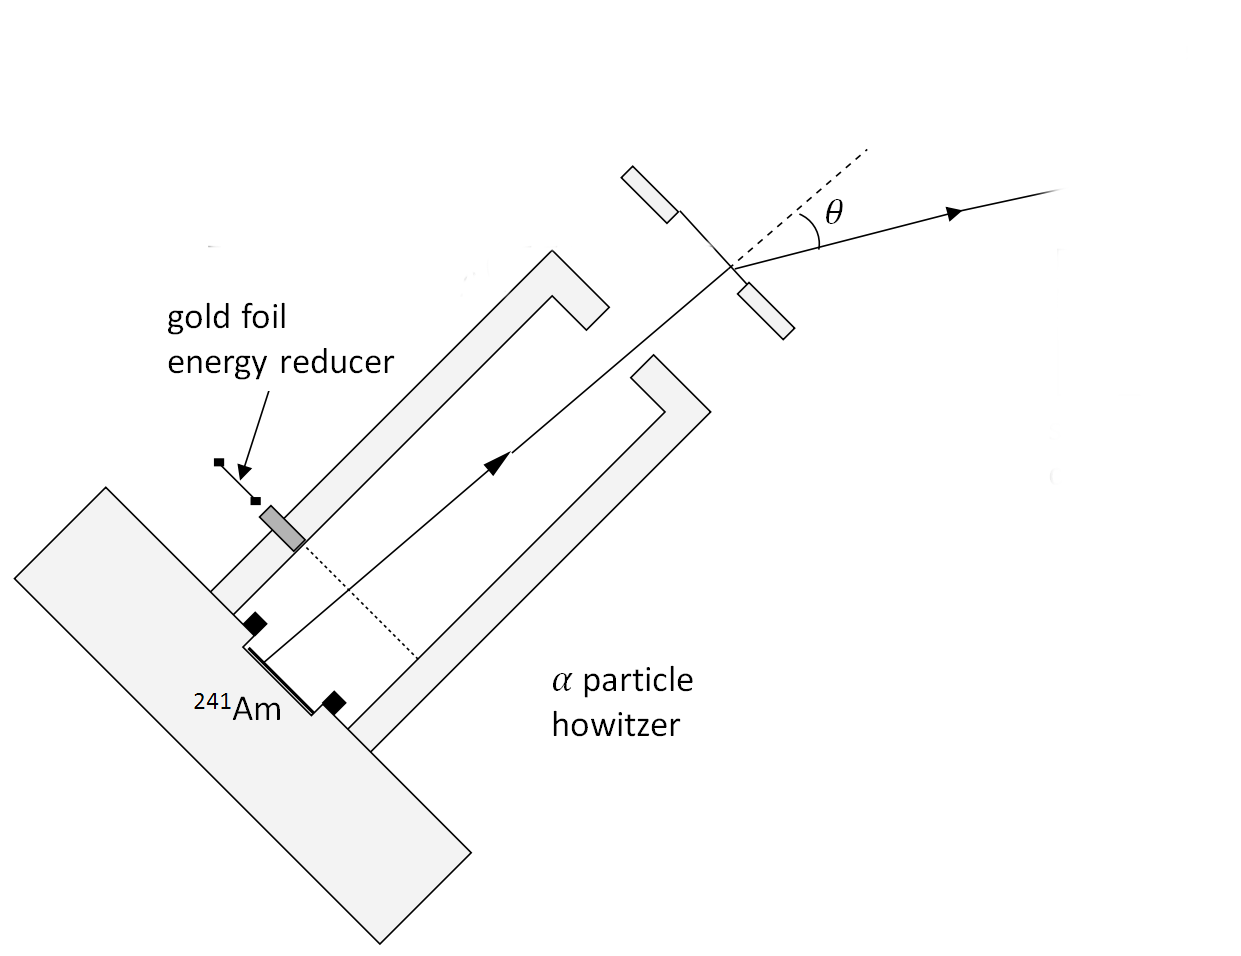
\includegraphics[width=0.8\textwidth]{apparatus-phi-detect}
\end{center}
\end{frame}

\begin{frame}
  \frametitle{Apparatus allows for scattering detection at various angles}
  \begin{center}
  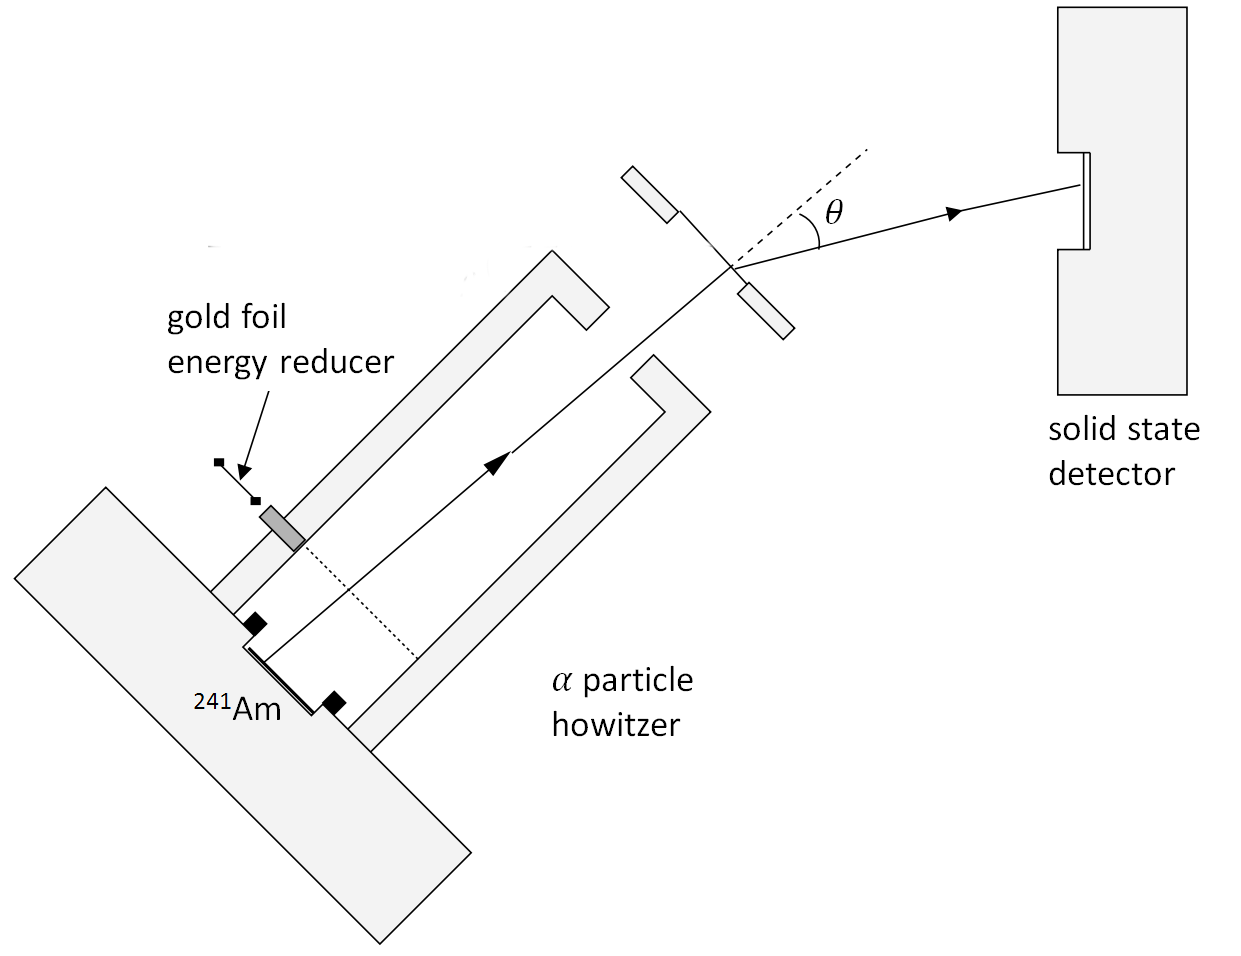
\includegraphics[width=0.8\textwidth]{apparatus-phi}
\end{center}
\end{frame}


\begin{frame}
  \frametitle{Apparatus allows for scattering detection at various angles}
  \begin{center}
  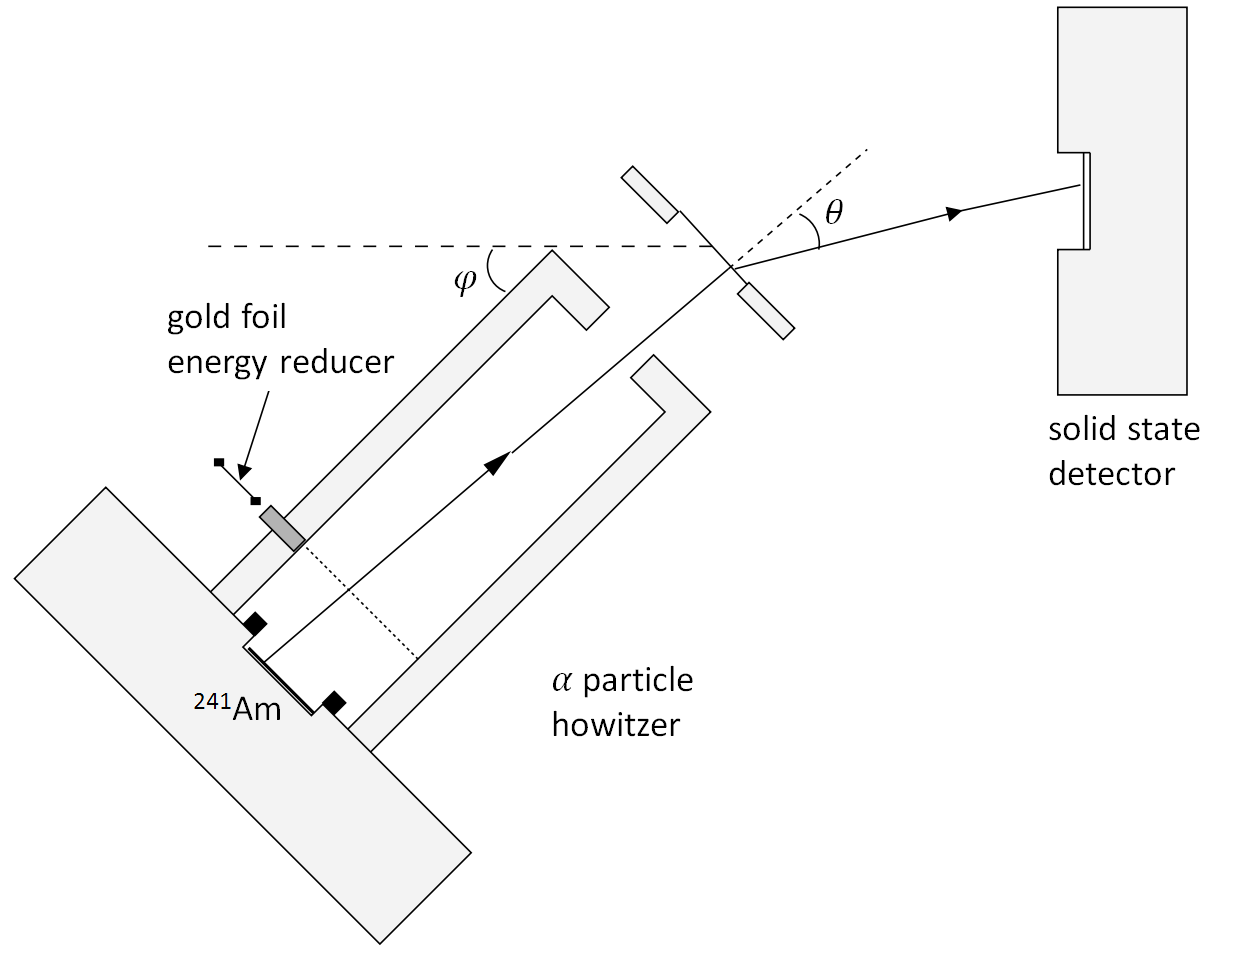
\includegraphics[width=0.8\textwidth]{apparatus}
\end{center}
\end{frame}

\begin{frame}
  \frametitle{Convolution of Angular Resolution Corrects for Beam/Detector Width}
  \begin{itemize}
    \item With the howitzer at an angle $\phi$, what is the probability of detecting a particle scattered between $\theta$ and $\theta + \dd{\theta}$?
      \pause
    \item Ideally, $P(\theta) = \delta(\theta-\phi)$.
      \pause
    \item Realistically, we expect roughly a triangle-shaped distribution.

  \end{itemize}
    \end{frame}

    \begin{frame}
      \frametitle{Beam Profile Indicates Both Angular Spread and Systematic Angular Offset }
      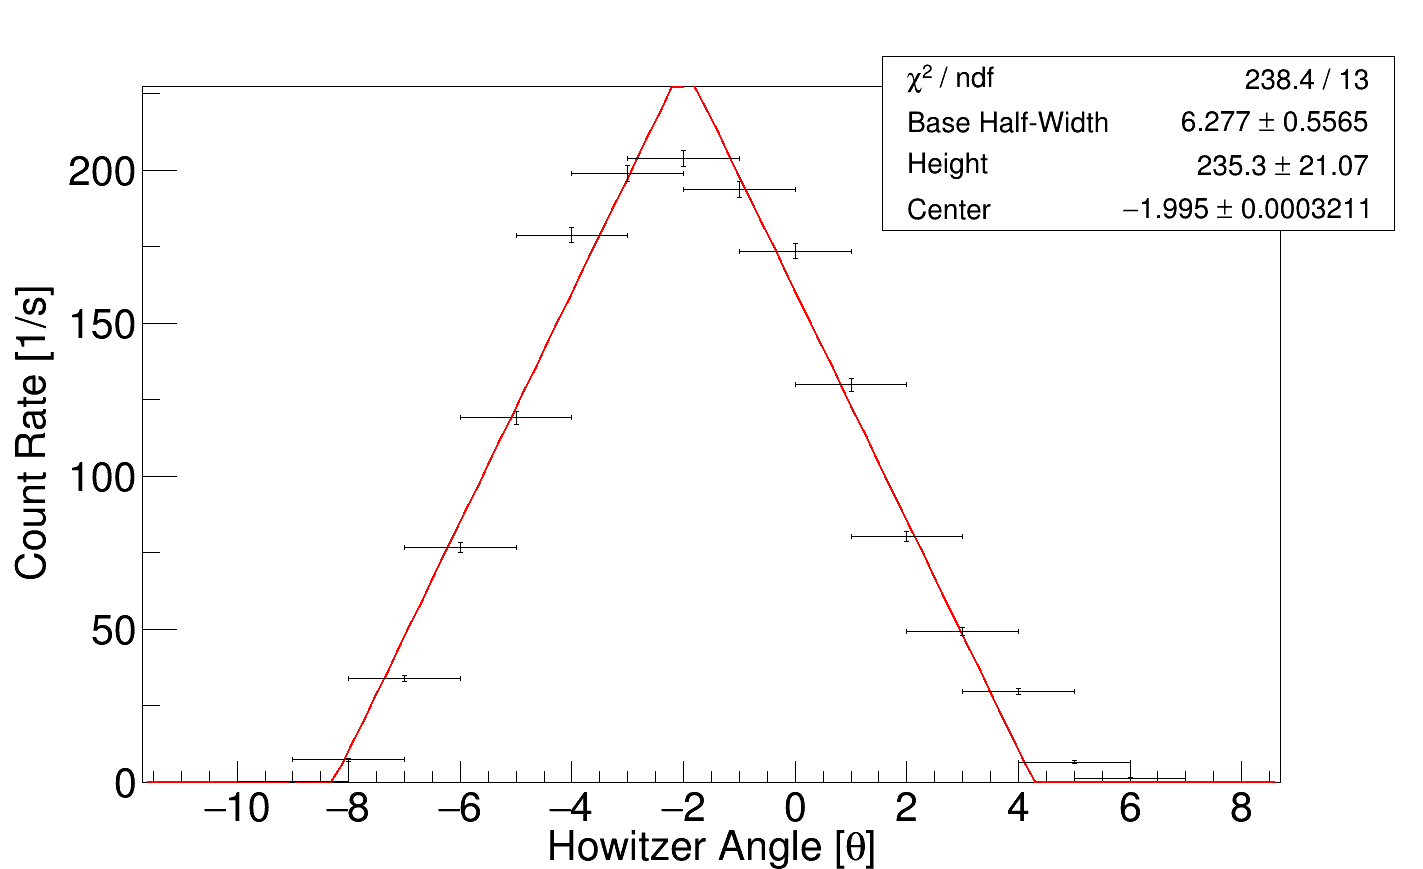
\includegraphics[width=1\textwidth]{c1.png}
    \end{frame}


\begin{frame}
  \frametitle{Convolving Beam Profile with Predicted Counting Rates Accounts for}
  \textbf{Rutherford}
  \begin{equation*}
    C_r(\phi) = C_{r,0}\int\limits_0^\pi g(\phi, \theta) \sin^{-4}(\theta/2) \dd{\theta}
  \end{equation*}
  \textbf{Thomson}
  \begin{equation*}
    C_t(\phi) = C_{t,0} \int\limits_0^\pi g(\phi, \theta) e^{-\frac{\theta^2}{\theta_0^2}}  \dd{\theta}
  \end{equation*}
\end{frame}

\begin{frame}
  \frametitle{MCA Readout Centered Around Energy Range}
  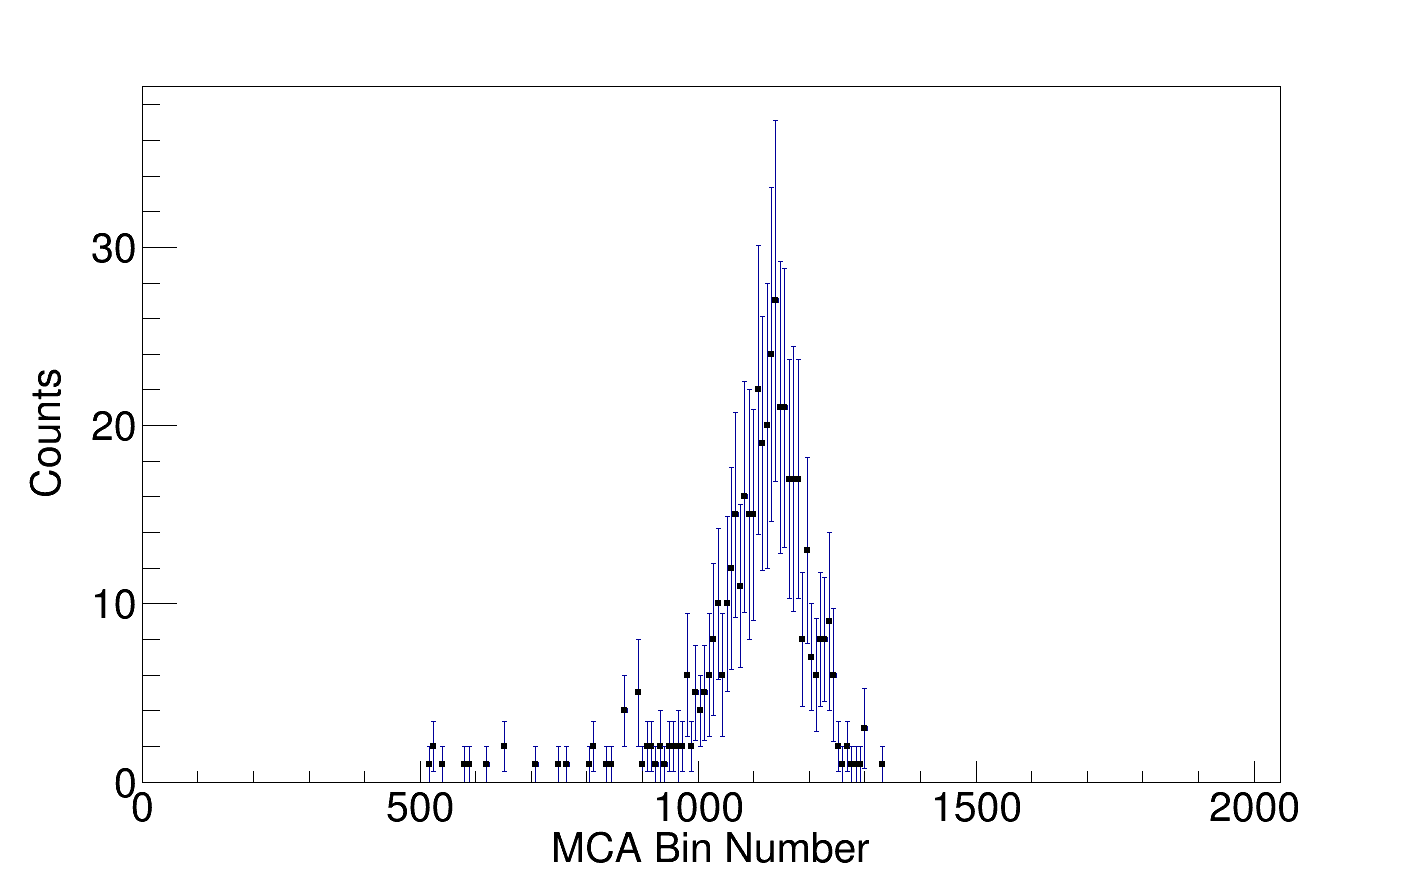
\includegraphics[width=1\textwidth]{mca_readout}
\end{frame}

    \begin{frame}
      \frametitle{Uncertainty in Angles and Counting Rates Contribute to Overall Uncertainty}
             \textbf{Noise}
      \pause
      \begin{itemize}
        \item Took measurements with the howitzer pointed away from the source to measure noise
          \pause
        \item Minimal noise detected, all at energies much less than our range of interest
      \end{itemize}
      \pause
      \textbf{Energy Distribution}
      \begin{itemize}
        \pause
    \item Landau distribution of energy loss allows us to consider all points as valid data
      \pause
    \item Count rate sill affected by counting uncertainty
  \end{itemize}
  \pause

 \textbf{Angular Uncertainty}
  \begin{itemize}
    \pause
  \item Protractor read by eye contributes $\pm 1$ degree uncertainty to angular measurements 
  \end{itemize}
\end{frame}

\begin{frame}
  \frametitle{Rutherford Scattering Effectively Predicts High-Angle Scattering}
    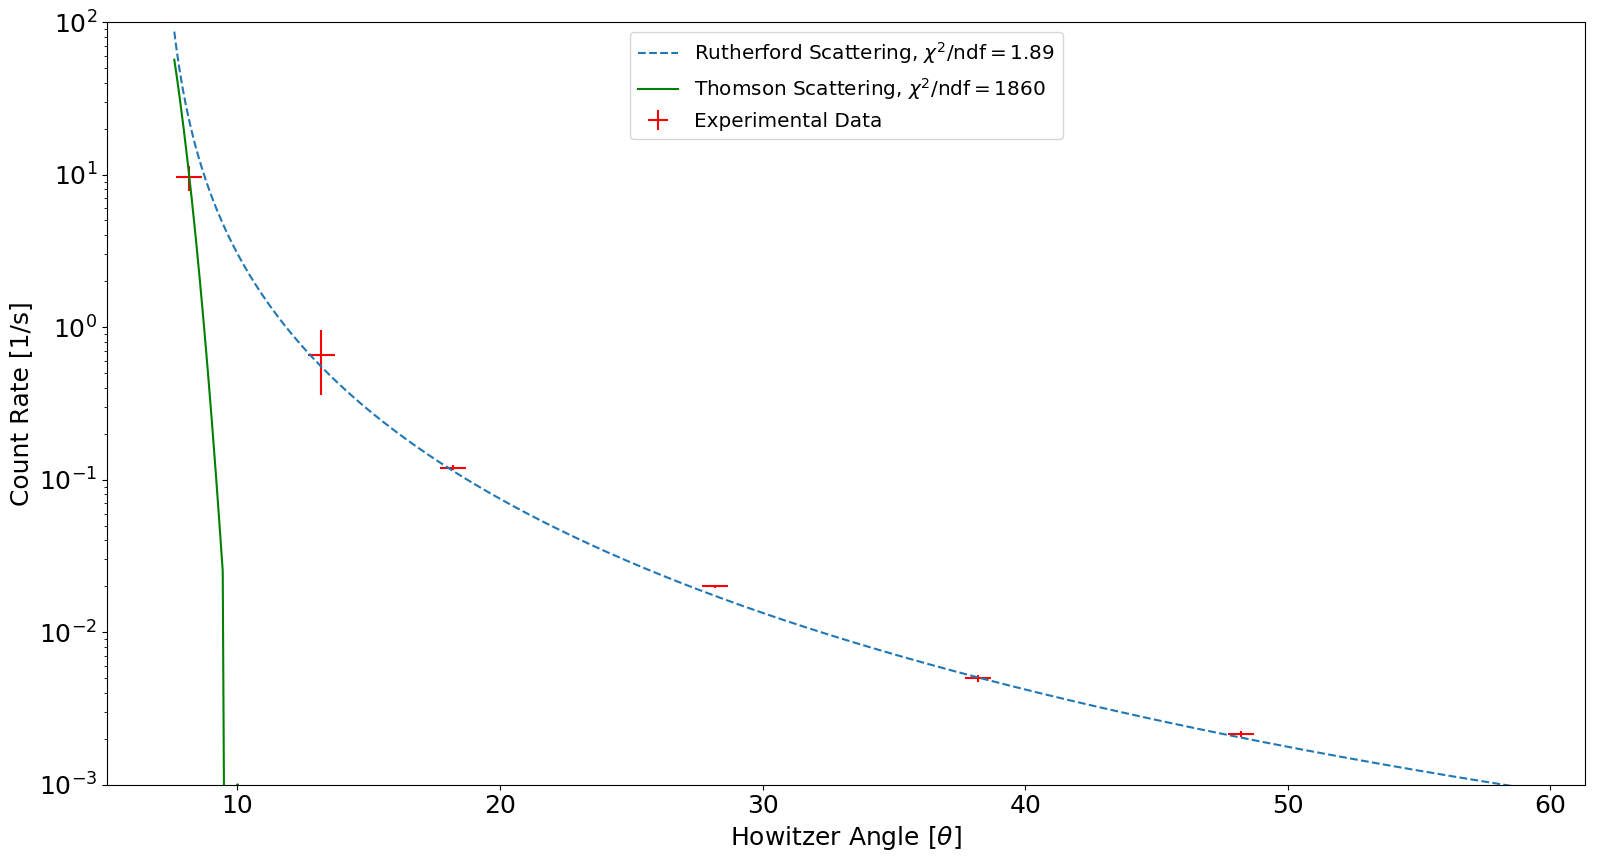
\includegraphics[width=1.0\textwidth]{convolve.png}
\end{frame}

\begin{frame}
\frametitle{Uncertainty in Convolution Contributes Small Uncertainty in $\chi^2/\text{ndf}$}
  \begin{table}
    \begin{tabular}{cc}
    Model & $\chi^2/\text{ndf}$ \\
    \hline
    Rutherford & $1.89 \pm 0.11$ \\
    Thomson & $1858 \pm 24$ \\
  \end{tabular}
  \end{table}
\end{frame}

\end{document}
